\documentclass{article}
\usepackage{lmodern}
\usepackage[T1]{fontenc}
\usepackage{shapepar}
\usepackage{microtype}
\usepackage{lipsum}
\usepackage{pgfplots}
\pgfplotsset{compat=1.9}
\usepackage{tikz}
\usetikzlibrary{calc,fit,intersections,folding}
\usepackage{pstricks-add}
\usetikzlibrary{arrows.meta,angles,arrows,quotes,backgrounds}

\newcommand{\tubecolor}{blue}
\newcommand{\thickness}{0.5mm}
\newcommand{\n}{2mm}


\begin{document}
\thispagestyle{empty}
\begin{center}
    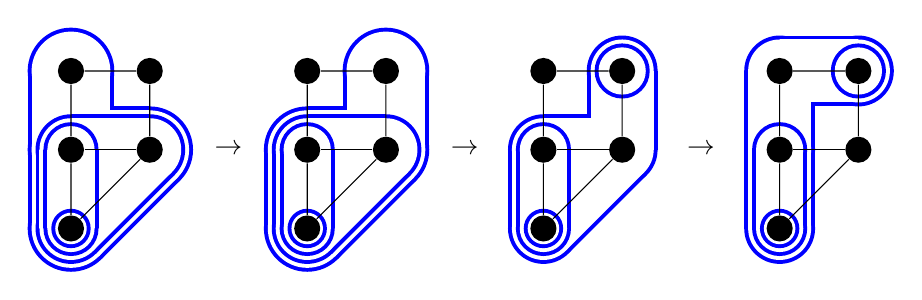
\begin{tikzpicture}
        \node [fill] (A) at (0,0) [circle] {};
        \node [fill ](B) at (0,1) [circle] {};
        \node [fill ](C) at (0,2) [circle] {};
        \node [fill ](D) at (1,1) [circle] {};
        \node [fill ](E) at (1,2) [circle] {};
        \draw (A) -- (B) -- (C) -- (E) -- (D) -- (A);
        \draw (B) -- (D);

        %Tube (A,B,C,D):
        \begin{scope}[on background layer]
            \fill[\tubecolor] (A) circle (\n + 7*\thickness);
            \fill[\tubecolor] (B) circle (\n + 7*\thickness);
            \fill[\tubecolor] (D) circle (\n + 7*\thickness);
            \fill[\tubecolor] (C) circle (\n + 7*\thickness);
            \draw[\tubecolor] [line width = 2*(\n + 7*\thickness)] (A.center) -- (B.center);
            \draw[\tubecolor] [line width = 2*(\n + 7*\thickness)] (A.center) -- (D.center);
            \draw[\tubecolor] [line width = 2*(\n + 7*\thickness)] (B.center) -- (D.center);
            \draw[\tubecolor] [line width = 2*(\n + 7*\thickness)] (B.center) -- (C.center);
            
            \fill[white] (A) circle (\n + 6*\thickness);
            \fill[white] (B) circle (\n + 6*\thickness);
            \fill[white] (D) circle (\n + 6*\thickness);
            \fill[white] (C) circle (\n + 6*\thickness);
            \draw[white] [line width = 2*(\n + 6*\thickness)] (A.center) -- (B.center);
            \draw[white] [line width = 2*(\n + 6*\thickness)] (A.center) -- (D.center);
            \draw[white] [line width = 2*(\n + 6*\thickness)] (B.center) -- (D.center);
            \draw[white] [line width = 2*(\n + 6*\thickness)] (B.center) -- (C.center);
        \end{scope}
        
        %Tube (A,B,D):
        \begin{scope}[on background layer]
            \fill[\tubecolor] (A) circle (\n + 5*\thickness);
            \fill[\tubecolor] (B) circle (\n + 5*\thickness);
            \fill[\tubecolor] (D) circle (\n + 5*\thickness);
            \draw[\tubecolor] [line width = 2*(\n + 5*\thickness)] (A.center) -- (B.center);
            \draw[\tubecolor] [line width = 2*(\n + 5*\thickness)] (A.center) -- (D.center);
            \draw[\tubecolor] [line width = 2*(\n + 5*\thickness)] (B.center) -- (D.center);

            \fill[white] (A) circle (\n + 4*\thickness);
            \fill[white] (B) circle (\n + 4*\thickness);
            \fill[white] (D) circle (\n + 4*\thickness);
            \draw[white] [line width = 2*(\n + 4*\thickness)] (A.center) -- (B.center);
            \draw[white] [line width = 2*(\n + 4*\thickness)] (A.center) -- (D.center);
            \draw[white] [line width = 2*(\n + 4*\thickness)] (B.center) -- (D.center);
            \fill[white] (A) -- (B) -- (D) -- (A);
        \end{scope}

        %Tube (A,B):
        \begin{scope}[on background layer]
            \fill[\tubecolor] (A) circle (\n + 3*\thickness);
            \fill[\tubecolor] (B) circle (\n + 3*\thickness);
            \draw[\tubecolor] [line width = 2*(\n + 3*\thickness)] (A.center) -- (B.center);

            \fill[white] (A) circle (\n + 2*\thickness);
            \fill[white] (B) circle (\n + 2*\thickness);
            \draw[line width = 2*(\n + 2*\thickness), white] (A.center) -- (B.center);
        \end{scope}
        
        %Tube (A):
        \begin{scope}[on background layer]
            \fill[\tubecolor] (A) circle (\n + \thickness);
            \fill[white] (A) circle (\n);
        \end{scope}
    \node at (2,1) {$\to$};
    \begin{scope}[xshift = 3cm]
        \node [fill] (A) at (0,0) [circle] {};
        \node [fill ](B) at (0,1) [circle] {};
        \node [fill ](E) at (0,2) [circle] {};
        \node [fill ](D) at (1,1) [circle] {};
        \node [fill ](C) at (1,2) [circle] {};
        \draw (A) -- (B) -- (E) -- (C) -- (D) -- (A);
        \draw (B) -- (D);

        %Tube (A,B,C,D):
        \begin{scope}[on background layer]
            \fill[\tubecolor] (A) circle (\n + 7*\thickness);
            \fill[\tubecolor] (B) circle (\n + 7*\thickness);
            \fill[\tubecolor] (D) circle (\n + 7*\thickness);
            \fill[\tubecolor] (C) circle (\n + 7*\thickness);
            \draw[\tubecolor] [line width = 2*(\n + 7*\thickness)] (A.center) -- (B.center);
            \draw[\tubecolor] [line width = 2*(\n + 7*\thickness)] (A.center) -- (D.center);
            \draw[\tubecolor] [line width = 2*(\n + 7*\thickness)] (B.center) -- (D.center);
            \draw[\tubecolor] [line width = 2*(\n + 7*\thickness)] (D.center) -- (C.center);
            
            \fill[white] (A) circle (\n + 6*\thickness);
            \fill[white] (B) circle (\n + 6*\thickness);
            \fill[white] (D) circle (\n + 6*\thickness);
            \fill[white] (C) circle (\n + 6*\thickness);
            \draw[white] [line width = 2*(\n + 6*\thickness)] (A.center) -- (B.center);
            \draw[white] [line width = 2*(\n + 6*\thickness)] (A.center) -- (D.center);
            \draw[white] [line width = 2*(\n + 6*\thickness)] (B.center) -- (D.center);
            \draw[white] [line width = 2*(\n + 6*\thickness)] (D.center) -- (C.center);
        \end{scope}
        
        %Tube (A,B,D):
        \begin{scope}[on background layer]
            \fill[\tubecolor] (A) circle (\n + 5*\thickness);
            \fill[\tubecolor] (B) circle (\n + 5*\thickness);
            \fill[\tubecolor] (D) circle (\n + 5*\thickness);
            \draw[\tubecolor] [line width = 2*(\n + 5*\thickness)] (A.center) -- (B.center);
            \draw[\tubecolor] [line width = 2*(\n + 5*\thickness)] (A.center) -- (D.center);
            \draw[\tubecolor] [line width = 2*(\n + 5*\thickness)] (B.center) -- (D.center);

            \fill[white] (A) circle (\n + 4*\thickness);
            \fill[white] (B) circle (\n + 4*\thickness);
            \fill[white] (D) circle (\n + 4*\thickness);
            \draw[white] [line width = 2*(\n + 4*\thickness)] (A.center) -- (B.center);
            \draw[white] [line width = 2*(\n + 4*\thickness)] (A.center) -- (D.center);
            \draw[white] [line width = 2*(\n + 4*\thickness)] (B.center) -- (D.center);
            \fill[white] (A) -- (B) -- (D) -- (A);
        \end{scope}

        %Tube (A,B):
        \begin{scope}[on background layer]
            \fill[\tubecolor] (A) circle (\n + 3*\thickness);
            \fill[\tubecolor] (B) circle (\n + 3*\thickness);
            \draw[\tubecolor] [line width = 2*(\n + 3*\thickness)] (A.center) -- (B.center);

            \fill[white] (A) circle (\n + 2*\thickness);
            \fill[white] (B) circle (\n + 2*\thickness);
            \draw[line width = 2*(\n + 2*\thickness), white] (A.center) -- (B.center);
        \end{scope}
        
        %Tube (A):
        \begin{scope}[on background layer]
            \fill[\tubecolor] (A) circle (\n + \thickness);
            \fill[white] (A) circle (\n);
        \end{scope}
    \node at (2,1) {$\to$};
    \end{scope}
    \begin{scope}[xshift = 6cm]
        \node [fill] (A) at (0,0) [circle] {};
        \node [fill ](B) at (0,1) [circle] {};
        \node [fill ](E) at (0,2) [circle] {};
        \node [fill ](D) at (1,1) [circle] {};
        \node [fill ](C) at (1,2) [circle] {};
        \draw (A) -- (B) -- (E) -- (C) -- (D) -- (A);
        \draw (B) -- (D);

        %Tube (A,B,C,D):
        \begin{scope}[on background layer]
            \fill[\tubecolor] (A) circle (\n + 5*\thickness);
            \fill[\tubecolor] (B) circle (\n + 5*\thickness);
            \fill[\tubecolor] (D) circle (\n + 5*\thickness);
            \fill[\tubecolor] (C) circle (\n + 5*\thickness);
            \draw[\tubecolor] [line width = 2*(\n + 5*\thickness)] (A.center) -- (B.center);
            \draw[\tubecolor] [line width = 2*(\n + 5*\thickness)] (A.center) -- (D.center);
            \draw[\tubecolor] [line width = 2*(\n + 5*\thickness)] (B.center) -- (D.center);
            \draw[\tubecolor] [line width = 2*(\n + 5*\thickness)] (D.center) -- (C.center);
            
            \fill[white] (A) circle (\n + 4*\thickness);
            \fill[white] (B) circle (\n + 4*\thickness);
            \fill[white] (D) circle (\n + 4*\thickness);
            \fill[white] (C) circle (\n + 4*\thickness);
            \draw[white] [line width = 2*(\n + 4*\thickness)] (A.center) -- (B.center);
            \draw[white] [line width = 2*(\n + 4*\thickness)] (A.center) -- (D.center);
            \draw[white] [line width = 2*(\n + 4*\thickness)] (B.center) -- (D.center);
            \draw[white] [line width = 2*(\n + 4*\thickness)] (D.center) -- (C.center);
        \end{scope}
        
        %Tube (C):
        \begin{scope}[on background layer]
            \fill[\tubecolor] (C) circle (\n + 3*\thickness);
            \fill[white] (C) circle (\n + 2*\thickness);
        \end{scope}
        %Tube (A,B):
        \begin{scope}[on background layer]
            \fill[\tubecolor] (A) circle (\n + 3*\thickness);
            \fill[\tubecolor] (B) circle (\n + 3*\thickness);
            \draw[\tubecolor] [line width = 2*(\n + 3*\thickness)] (A.center) -- (B.center);

            \fill[white] (A) circle (\n + 2*\thickness);
            \fill[white] (B) circle (\n + 2*\thickness);
            \draw[line width = 2*(\n + 2*\thickness), white] (A.center) -- (B.center);
        \end{scope}
        
        %Tube (A):
        \begin{scope}[on background layer]
            \fill[\tubecolor] (A) circle (\n + \thickness);
            \fill[white] (A) circle (\n);
        \end{scope}
        \node at (2,1) {$\to$};
    \end{scope}
    
    \begin{scope}[xshift = 9cm]
        \node [fill] (A) at (0,0) [circle] {};
        \node [fill ](B) at (0,1) [circle] {};
        \node [fill ](E) at (0,2) [circle] {};
        \node [fill ](D) at (1,1) [circle] {};
        \node [fill ](C) at (1,2) [circle] {};
        \draw (A) -- (B) -- (E) -- (C) -- (D) -- (A);
        \draw (B) -- (D);

        %Tube (A,B,C,D):
        \begin{scope}[on background layer]
            \fill[\tubecolor] (A) circle (\n + 5*\thickness);
            \fill[\tubecolor] (B) circle (\n + 5*\thickness);
            \fill[\tubecolor] (E) circle (\n + 5*\thickness);
            \fill[\tubecolor] (C) circle (\n + 5*\thickness);
            \draw[\tubecolor] [line width = 2*(\n + 5*\thickness)] (A.center) -- (B.center);
            \draw[\tubecolor] [line width = 2*(\n + 5*\thickness)] (B.center) -- (E.center);
            \draw[\tubecolor] [line width = 2*(\n + 5*\thickness)] (E.center) -- (C.center);
            
            \fill[white] (A) circle (\n + 4*\thickness);
            \fill[white] (B) circle (\n + 4*\thickness);
            \fill[white] (E) circle (\n + 4*\thickness);
            \fill[white] (C) circle (\n + 4*\thickness);
            \draw[white] [line width = 2*(\n + 4*\thickness)] (A.center) -- (B.center);
            \draw[white] [line width = 2*(\n + 4*\thickness)] (B.center) -- (E.center);
            \draw[white] [line width = 2*(\n + 4*\thickness)] (E.center) -- (C.center);
        \end{scope}
        
        %Tube (C):
        \begin{scope}[on background layer]
            \fill[\tubecolor] (C) circle (\n + 3*\thickness);
            \fill[white] (C) circle (\n+2*\thickness);
        \end{scope}
        %Tube (A,B):
        \begin{scope}[on background layer]
            \fill[\tubecolor] (A) circle (\n + 3*\thickness);
            \fill[\tubecolor] (B) circle (\n + 3*\thickness);
            \draw[\tubecolor] [line width = 2*(\n + 3*\thickness)] (A.center) -- (B.center);

            \fill[white] (A) circle (\n + 2*\thickness);
            \fill[white] (B) circle (\n + 2*\thickness);
            \draw[line width = 2*(\n + 2*\thickness), white] (A.center) -- (B.center);
        \end{scope}
        
        %Tube (A):
        \begin{scope}[on background layer]
            \fill[\tubecolor] (A) circle (\n + \thickness);
            \fill[white] (A) circle (\n);
        \end{scope}
    \end{scope}
    
    \end{tikzpicture}
    \end{center}

\end{document}